% 文档类设置
\documentclass{ctexart}

% 导入宏包
\usepackage{hyperref} % PDF标签
\usepackage{graphicx} % 图片
\graphicspath{{images/}} % 图片路径
\usepackage{geometry} % 页面边距宏包
\geometry{left=3.17cm,right=3.17cm,top=2.54cm,bottom=2.54cm} % 页边距
\usepackage{fancyhdr} % 页眉页脚
\pagestyle{fancy} % 页面样式
\cfoot{\thepage} % 页脚中部
\renewcommand\headrulewidth{0pt}%隐藏页眉横线
\usepackage{enumerate} % 编号列表
\usepackage[simplified]{pgf-umlcd} % UML
\usepackage{listings} % 代码排版
\usepackage{dirtree} % 绘制树形目录
\usepackage{url} % 超链接
\usepackage{color,xcolor} % 颜色宏包
\usepackage[ruled]{algorithm2e} % 算法环境
% \usepackage{algorithmic} % 算法描述
% 代码块风格
\lstset{
    numbers=left,           % 行号
    numberstyle=\tiny,      % 行号样式
    basicstyle=\ttfamily,   % 基本代码风格
    breaklines=true,        % 自动换行
    keywordstyle=\bfseries\color{green!40!black}, % 关键字风格
    commentstyle=\itshape\color{gray}, % 注释的风格
    identifierstyle=\bfseries\color{blue}, % 标识符风格
    stringstyle=\color{orange}, % 字符串风格
    columns=fixed,
    frame=single, % 显示边框
    xleftmargin=\parindent,  % 左边距
    % xrightmargin=\parindent, % 右边距
    aboveskip=1em, % 顶部间隔
    captionpos=b % 文字提示符
}
\renewcommand{\lstlistingname}{代码}

% 算法描述的设置
\SetAlgorithmName{算法}{算法}{算法列表}
\SetKwInput{KwIn}{输入}
\SetKwInput{KwOut}{输出}
\LinesNumbered


% 角注设置
% \renewcommand{\thefootnote}{\fnsymbol{footnote}}

% 章节标题设置
\ctexset{
    section = {
        format+ =  \zihao{-3} \raggedright,
        name = {,\quad},
        number = \arabic{section},
        aftername = \hspace{0pt}
    },
    subsection = {
        format+ =  \zihao{4} \raggedright,
        name = {,\quad},
        number = \arabic{section}.\arabic{subsection},
        aftername = \hspace{0pt}
    },
    subsubsection = {
        format+ =  \zihao{-4} \raggedright,
        name = {,\quad},
        number = \arabic{section}.\arabic{subsection}.\arabic{subsubsection},
        aftername = \hspace{0pt}
    }
}

% 封面页
\newcommand{\makecover}[4]{
    \begin{titlepage}
        \centering
        
\includegraphics[width=0.5\textwidth]{logo.png}\par
        \vspace{1cm}
        {\kaishu\ziju{0.1}\Huge 数学与计算机学院}\par
        \vspace{5.5cm}
        {\bfseries\ziju{0.1}\zihao{-0} #1}\par
        \vspace{5.5cm}
        {\kaishu\ziju{0.1}\Huge #2}\par
        \vspace{0.7cm}
        {\kaishu\Large #3}\par
        \vspace{1em}
        {\kaishu\large #4}\par
        \vspace{4em}
        {\itshape 本作品采用 \href{https://creativecommons.org/licenses/by-nc-sa/4.0/}{CC-BY-NC-SA} 协议进行许可}\par
        \vspace{1em}
        
\includegraphics[width=0.2\textwidth]{cc-by-nc-sa.png}
    \end{titlepage}
}

% 画UML类图
% 参数2:文本宽度,参数3:类名,参数1:左上角坐标
\newenvironment{UMLClass}[3][0,0]
{
    \vspace{1em}\par\ttfamily
    \begin{tikzpicture}
        \begin{class}[text width=#2]{#3}{#1}
}
{
        \end{class}
    \end{tikzpicture}
    \vspace{1em}
}


\begin{document}
    % 产生封面
    \makecover{停车场管理系统设计报告}{杨鑫}{计算机11902班}{\today}
    
    \section{需求分析}

    \subsection{问题描述}
    停车场内只有一个可停放 $n$ 辆汽车的狭长通道,且只有一个大门可供汽车进出。
    
    汽车在停车场内按车辆到达时间的先后顺序,依次由北向南排列(大门在最南端,
    最先到达的第一辆车停放在停车场的最北端),若车场内已停满 $n$ 辆汽车,
    则后来的汽车只能在门外的便道上等候,一旦有车开走,则排在便道上的第一辆车即可开入。

    当停车场内某辆车要离开时,在它之后开入的车辆必须先退出车场为它让路,
    待该辆车开出大门外,其它车辆再按原次序进入车场,
    每辆停放在车场的车在它离开车场时必须按它停留的时间长短交纳费用。
    
    试为停车场编制按上述要求进行管理的模拟程序。
    
    \subsection{基本要求}
    \begin{enumerate}[\indent (1)]
        \item 以栈模拟停车场,以队列模拟车场外的便道,
              按照从终端读入的输入数据序列进行模拟管理;
        \item 每一组输入数据包括三个数据项:汽车“到达”或“离去”信息、
              汽车牌照号码及到达或离去的时刻,对每一组输入数据进行操作后的输出数据为:
              若是车辆到达,则输出汽车在停车场内或便道上的停车位置;
              若是车离去,则输出汽车在停车场内停留的时间和应交纳的
              费用(在便道上停留的时间不收费);
        \item 栈以顺序结构实现,队列以链表实现。
    \end{enumerate}
    
    \section{概要设计}

    \subsection{数据结构}

    \subsubsection{时间类}
    时间是进行收费的依据,此处假定时间在一天之内。时间类既可以表示一个时刻,
    也可以表示一段时间长度。
    
    时间类数据成员:
    \begin{itemize}\ttfamily
        \item hour:指示时钟
        \item minute:指示分钟
    \end{itemize}

    时间类成员函数:
    \begin{itemize}\ttfamily
        \item Time:构造函数
        \item operator+=:进行时间的复合加法,即将相加后的结果赋给当前对象,并返回当前对象
        \item operator-=:进行时间的复合减法,即将相减后的结果赋给当前对象,并返回当前对象
    \end{itemize}

    \begin{center}
        \begin{UMLClass}{13cm}{Time}
            \attribute{+ hour: int}
            \attribute{+ minute: int}
            \operation{+ Time()}
            \operation{+ Time(hour: int, minute: int)}
            \operation{<<friend>> operator+(left: const Time\&, right: const Time\&): Time}
            \operation{+ operator+=(right: const Time\&): Time}
            \operation{<<friend>> operator-(left: const Time\&, right: const Time\&): Time}
            \operation{+ operator-=(right: const Time\&): Time}
            \operation{<<friend>> operator==(left: const Time\&, right: const Time\&): bool}
            \operation{<<friend>> operator<(left: const Time\&, right: const Time\&): bool}
            \operation{<<friend>> operator<=(left: const Time\&, right: const Time\&): bool}
            \operation{<<friend>> operator>(left: const Time\&, right: const Time\&): bool}
            \operation{<<friend>> operator>=(left: const Time\&, right: const Time\&): bool}
            \operation{<<friend>> operator<<(os: ostream\&, t: const Time\&): ostream\&}
        \end{UMLClass}
    \end{center}

    时间类非成员函数:
    \begin{itemize}\ttfamily
        \item operator+:时间加法
        \item operator-:时间减法
        \item operator==:判断时间是否相等
        \item operator<:判断前一个时间是否小于后一个时间
        \item operator<=:判断前一个时间是否小于等于后一个时间
        \item operator>:判断前一个时间是否大于后一个时间
        \item operator>=:判断前一个时间是否大于等于后一个时间
        \item operator<<:将时间输出到输出流中
    \end{itemize}

    \subsubsection{汽车类}
    汽车是后续操作的基础元素,结合题目要求,汽车应包含牌照号码、停车时间等数据。

    汽车类数据成员:
    \begin{itemize}\ttfamily
        \item number:汽车牌照号码
        \item lastTime:最后一次在停车场(栈)内的时刻
        \item parking: 停车时间
    \end{itemize}
    
    lastTime 和 parking 并非实时更新,而是当有车辆到达或离去时才会做相应的改变。

    \begin{center}
        \begin{UMLClass}{13cm}{Car}
            \attribute{- number: string}
            \attribute{- lastTime: Time}
            \attribute{- parking: Time}
            \operation{+ Car()}
            \operation{+ Car(number: string)}
            \operation{+ operation==(car: const Car\&): bool}
            \operation{+ updateLastTime(time: const Time\&)}
            \operation{+ setLastTime(time: const Time\&)}
            \operation{+ getLastTime(): Time}
            \operation{+ addParkingTime(time: const Time\&)}
            \operation{<<friend>> operator<<(os: ostream\&, t: const Car\&): ostream\&}
        \end{UMLClass}
    \end{center}

    汽车类成员函数:
    \begin{itemize}\ttfamily
        \item Car:构造函数
        \item operation==:判断是否为同一辆汽车(只判断牌照号码)
        \item updateLastTime:设置最后一次在停车场(栈)内的时刻,并增加停车时间
        \item setLastTime:设置最后一次在停车场(栈)内的时刻
        \item getLastTime:获取最后一次在停车场(栈)内的时刻
        \item addParkingTime:增加停车时间
        \item getParingTime:获取停车时间
    \end{itemize}

    汽车类非成员函数:
    \begin{itemize}\ttfamily
        \item operator<<:将汽车信息输出到输出流中
    \end{itemize}
    
    \subsubsection{栈类模板}
    栈是一种“先进后出”的数据结构,此处用于组织停车场内汽车的停放。

    我们选用线性结构实现栈,并进行模板化,以便下次复用。

    模板参数T\footnotemark[1],表示基础元素类型,在编写代码时,可设为Car。
    
    \footnotetext[1]{
     从模板参数T,定义出以下几种嵌套类型:
     \begin{itemize}
         \item $T \longrightarrow value\_type$,基础元素类型
         \item $T* \longrightarrow pointer$,指针
         \item $const\ T* \longrightarrow const\_pointer$,常指针
         \item $T\& \longrightarrow reference$,引用
         \item $const\ T\& \longrightarrow const\_reference$,常引用
     \end{itemize} 
     }

     \begin{center}
        \begin{UMLClass}{10cm}{Stack<T>}
            \attribute{- \_top: pointer}
            \attribute{- \_base: pointer}
            \attribute{- \_cap: pointer}
            \operation{+ Stack()}
            \operation{$\sim$ Stack()}
            \operation{+ operator[](pos: size\_type): reference}
            \operation{+ operator[](pos: size\_type): const\_reference}
            \operation{+ top(): reference}
            \operation{+ top(): const\_reference}
            \operation{+ empty(): bool}
            \operation{+ size(): size\_type}
            \operation{+ capacity(): size\_type}
            \operation{+ push(data: const\_reference)}
            \operation{+ pop()}
            \operation{+ index(data: const\_reference): size\_type}
            \operation{+ print()}
            \operation{+ reserve(newCapacity: size\_type)}
        \end{UMLClass}
        \footnote{size\_type是无符号超长整型,源于std::size\_t。}
    \end{center}

    栈类数据成员:
    \begin{itemize}\ttfamily
        \item \_top 栈顶
        \item \_base 栈底
        \item \_cap 当前栈存储空间的尾部
    \end{itemize}
    
    特别指出,栈顶指针\_top,其初值指向栈底,即\_top == \_base可作为栈空的标记,
    每当插入新的栈顶元素时,指针\_top增1;删除栈顶元素时,指针\_top减1,因此,非空栈中的
    栈顶指针始终在栈顶元素的下一个位置上。
    
    \_cap指针则仅指示当前栈存储空间的尾部,其真实地址则是尾部的下一个位置。

    这两种设计都是为了方便程序的编写。

    栈类成员函数:
    \begin{itemize}\ttfamily
        \item Stack:构造函数
        \item $\sim$Stack:析构函数
        \item operator[]:访问器\footnote{设置访问器仅用于方便本次项目的代码编写,破坏了栈的设计原则,在编写一般程序时,不应在栈中设置访问器。}
        \item top:访问栈顶
        \item empty:判断栈是否为空
        \item size:获取栈长
        \item capacity:获取栈的存储容量
        \item push:入栈
        \item pop:出栈
        \item index:寻找元素的第一个位置
        \item print:打印栈
        \item reserve:重新分配存储空间容量
    \end{itemize}

    \subsubsection{队列类模板}
    队列,是一种“先进先出”的数据结构,此处可用于模拟停车场外的便道。
    
    我们选用链式结构实现队列,并进行模板化,以便下次复用。

    模板参数T\footnotemark[1],表示基础元素类型,在编写代码时,可设为Car。

    \footnotetext[1]{
        从模板参数T定义出的嵌套类型与Stack类相似,但增加了4个嵌套定义:
        \begin{itemize}
            \item $QNode<T>* \longrightarrow node\_ptr$,节点指针
            \item $const\ QNode<T>* \longrightarrow const\_node\_ptr$,节点常指针
            \item $QNode<T>\& \longrightarrow node\_ref$,节点引用
            \item $const\ QNode<T>\& \longrightarrow const\_node\_ref$,节点常引用
        \end{itemize}
    }

    首先设计一个队列节点类,与链表节点类似:

    \begin{center}
        \begin{UMLClass}{13cm}{QNode<T>}
            \attribute{- \_data: value\_type}
            \attribute{- \_next: node\_ptr}
            \operation{+ QNode()}
            \operation{+ QNode(data: const\_reference, next = nullptr: const\_node\_ptr)}
            \operation{+ data(): reference}
            \operation{+ data(): const\_reference}
            \operation{+ setData(data: const\_reference)}
            \operation{+ next(): node\_ptr}
            \operation{+ next(): const\_node\_ptr}
            \operation{+ setNext(next: const\_node\_ptr)}
        \end{UMLClass}
    \end{center}

    队列节点类数据成员:
    \begin{itemize}\ttfamily
        \item \_data:数据域
        \item \_next:指针域,指向下一节点
    \end{itemize}

    队列节点类成员函数:
    \begin{itemize}\ttfamily
        \item QNode:构造函数
        \item data:返回数据域
        \item setData:设置数据域
        \item next:返回下一节点
        \item setNext:设置下一节点
    \end{itemize}

    然后以队列节点为基础设计队列类模板:

    \begin{center}
        \begin{UMLClass}{8cm}{Queue<T>}
            \attribute{- \_front: node\_ptr}
            \attribute{- \_back: node\_ptr}
            \operation{+ Queue()}
            \operation{$\sim$ Queue()}
            \operation{+ front(): reference}
            \operation{+ front(): const\_reference}
            \operation{+ back(): reference}
            \operation{+ back(): const\_reference}
            \operation{+ empty(): bool}
            \operation{+ size(): size\_type}
            \operation{+ push(data: const\_reference)}
            \operation{+ pop()}
            \operation{+ erase(data: const\_reference)}
            \operation{+ print()}
        \end{UMLClass}
    \end{center}

    队列类数据成员:
    \begin{itemize}\ttfamily
        \item \_front:队头指针
        \item \_back:队尾指针
    \end{itemize}

    队列类成员函数:
    \begin{itemize}\ttfamily
        \item Queue:构造函数
        \item $\sim$ Queue:析构函数
        \item front:返回队头
        \item back:返回队尾
        \item empty:返回队列是否为空
        \item size:返回队列的大小
        \item push:入队列
        \item pop:出队列
        \item erase:直接擦除第一个值为data的节点\footnote[1]{设计此函数仅用于方便本项目代码的编写,破坏了队列的设计原则,在编写一般程序时,不应在队列中设置此函数。}
        \item print:打印队列
    \end{itemize}
    \subsubsection{停车场类}
    
    依据题意,整个停车场包含一个有限容量的停车场(栈)和场外的便道(队列)。

    将栈和队列综合,封装成一个停车场类。

    \begin{center}
        \begin{UMLClass}{13cm}{ParkLot}
            \attribute{- s: Stack<Car>}
            \attribute{- q: Queue<Car>}
            \attribute{- size: size\_t}
            \operation{+ ParkLot()}
            \operation{+ ParkLot(size: size\_t)}
            \operation{+ add(carNumber: const string\&, arriveTime: const Time\&)}
            \operation{+ reduce(carNumber: const string\&, leaveTime: const Time\&)}
            \operation{+ print()}
        \end{UMLClass}
    \end{center}

    停车场类数据成员:
    \begin{itemize}\ttfamily
        \item s:停车场(栈)
        \item q:便道(队列)
        \item size:停车场容量(栈最大大小)
    \end{itemize}

    停车场类函数成员:
    \begin{itemize}\ttfamily
        \item ParkLot:构造函数
        \item add:到达汽车
        \item reduce:离开汽车
        \item print:打印停车场
    \end{itemize}
    \subsection{程序模块}
    绝大部分算法均已经在各数据结构中实现。

    下面设计车辆收费算法。

    假定:

    车辆仅收取在停车场(栈)上停留的费用,在便道(队列)上停留的时间不收费。

    \begin{enumerate}[\indent 1、]
        \item 停留时间小于1小时,不收费;
        \item 停留时间在1小时以上,2小时以下,收费5元;
        \item 停留时间在2小时以上,2小时以上的部分,每小时收取3元(不满1小时,按1小时计算)。
    \end{enumerate}

    例如:

    停留半小时,不收费;

    停留1个半小时,收费5元;

    停留4个小时,收费11元。
    \section{详细设计}

    \subsection{类的函数实现}
    \subsubsection{时间类}
    时间类的函数实现如代码\ref{code1}所示。
\begin{lstlisting}[language=C++,caption=Time类的实现,label=code1]
struct Time {
    /************** 公有数据成员 **************/
    int hour;   // 时
    int minute; // 分

    // 构造函数
    Time() : Time(0, 0) {}

    Time(int hour, int minute) {
        this->hour = hour;
        this->minute = minute;
    }

    friend Time operator+(const Time &left, const Time &right);
    friend Time operator-(const Time &left, const Time &right);
    friend bool operator==(const Time &left, const Time &right);
    friend bool operator<(const Time &left, const Time &right);
    friend bool operator<=(const Time &left, const Time &right);
    friend bool operator>(const Time &left, const Time &right);
    friend bool operator>=(const Time &left, const Time &right);
    friend std::ostream &operator<<(std::ostream &os, const Time &t);

    Time operator+=(const Time &right) {
        *this = *this + right;
        return *this;
    }

    Time operator-=(const Time &right) {
        *this = *this - right;
        return *this;
    }
};

Time operator+(const Time &left, const Time &right) {
    int m = (left.minute + right.minute) % 60;
    int h = left.hour + right.hour + (left.minute + right.minute) / 60;
    return Time{h, m};
}

Time operator-(const Time &left, const Time &right) {
    if (left.hour < right.hour ||
        left.hour == right.hour && left.minute < right.minute)
        return Time{0, 0};

    int h = left.hour - right.hour;
    int m = left.minute - right.minute;
    if (m < 0) {
        m += 60;
        h--;
    }
    return Time(h, m);
}

bool operator==(const Time &left, const Time &right) {
    return left.hour == right.hour && left.minute == right.minute;
}

bool operator<(const Time &left, const Time &right) {
    if (left.hour < right.hour)
        return true;
    else if (left.hour == right.hour) {
        return left.minute < right.minute;
    } else
        return false;
}

bool operator<=(const Time &left, const Time &right) {
    return left == right || left < right;
}

bool operator>(const Time &left, const Time &right) {
    return !(left <= right);
}

bool operator>=(const Time &left, const Time &right) {
    return !(left < right);
}

// 将时间输出到流中
std::ostream &operator<<(std::ostream &os, const Time &t) {
    os << t.hour << "h " << t.minute << "m";
    return os;
} 
\end{lstlisting}

    \subsubsection{汽车类}
    汽车类的函数实现如代码\ref{code2}所示。
\begin{lstlisting}[language=C++,caption=Car类的实现,label=code2]
class Car {
    private:
        /************** 私有数据成员 **************/
        std::string number; // 牌照号码
        Time lastTime;      // 最后一次在栈内的时刻
        Time parking;       // 停车时间
    
    public:
        // 构造函数
        Car() = default;
    
        explicit Car(std::string number) {
            this->number = number;
            this->parking = {0, 0};
        }
    
        // 判断是否为同一辆车
        bool operator==(const Car &car) {
            return this->number == car.number;
        }
    
        // 设置最后一次在栈内的时刻,并增加停车时间
        void updateLastTime(const Time &time) {
            addParkingTime(time - lastTime);
            this->lastTime = time;
        }
    
        // 设置最后一次在栈内的时刻
        void setLastTime(const Time &time) {
            this->lastTime = time;
        }
    
        // 获取最后一次在栈内的时刻
        Time getLastTime() {
            return lastTime;
        }
    
        // 增加停车时间
        void addParkingTime(const Time &time) {
            this->parking += time;
        }
    
        // 获取停车时间
        Time getParingTime() {
            return parking;
        }
    
        friend std::ostream &operator<<(std::ostream &os, const Car &c);
    };
    
    // 将汽车输出到流中
    std::ostream &operator<<(std::ostream &os, const Car &c) {
        os << c.number;
        return os;
    }
\end{lstlisting}
    \subsubsection{栈类模板}
    栈类模板的函数实现如代码\ref{code3}所示。
\begin{lstlisting}[language=C++,caption=Stack类的实现,label=code3]
template<typename T>
class Stack {
public:
    /************** 嵌套类型 **************/
    typedef T           value_type;         // 基础元素类型
    typedef T*          pointer;            // 指针
    typedef const T*    const_pointer;      // 常指针
    typedef T&          reference;          // 引用
    typedef const T&    const_reference;    // 常引用
    typedef std::size_t size_type;          // 无符号长整型

private:
    /************** 私有数据成员 **************/
    pointer _top;  // 栈顶(后一位)
    pointer _base; // 栈底
    pointer _cap;  // 当前栈存储空间的尾部(后一位)

public:
    // 构造一个空栈
    Stack() {
        try {
            _base = new value_type[Stack_Init_Size];
            _top = _base;
            _cap = _base + Stack_Init_Size;
        } catch (std::bad_alloc &) { // 分配内存异常
            std::cerr << "Exception: Can not construct a new Stack object,"
                        << "because there is no available memory."
                        << std::endl;
        }
    }

    // 销毁栈
    ~Stack() {
        delete[] _base;
        _base = _top = _cap = nullptr;
    }

    // 返回pos位置的引用
    reference operator[](size_type pos) {
        assert(!empty());
        return *(_base + pos);
    }

    // 返回pos位置的常引用
    const_reference operator[](size_type pos) const {
        assert(!empty());
        return *(_base + pos);
    }

    // 返回栈顶的引用
    reference top() {
        assert(!empty());
        return *(_top - 1);
    }

    // 返回栈顶的常引用
    const_reference top() const {
        assert(!empty());
        return *(_top - 1);
    }

    // 返回栈是否为空
    bool empty() const noexcept {
        return _top == _base;
    }

    // 获取栈长
    size_type size() const noexcept {
        return (_top - _base);
    }

    // 获取栈的存储容量
    size_type capacity() const noexcept {
        return _cap - _base;
    }

    // 入栈
    void push(const_reference data) {
        if (size() >= capacity())
            try {
                reserve(capacity() * 3 / 2);
            } catch (std::bad_alloc &) {
                std::cerr << "Exception: Can not push new data,"
                            << "because there is no available memory."
                            << std::endl;
            }
        *(_top++) = data;
    }

    // 出栈
    void pop() {
        assert(!empty());
        _top--;
    }

    // 寻找元素的第一个位置
    size_type index(const_reference data) {
        for (size_type i = 0; i < size(); i++) {
            if (*(_base + i) == data)
                return i;
        }
        throw std::out_of_range{"not found"};
    }

    // 打印栈
    void print() {
        if (empty())
            std::cout << "null" << std::endl;
        else {
            for (size_type i = 0; i < size(); i++) {
                std::string ch = ((i + 1) % 5 ? " " : "\n");
                if (i + 1 == size())
                    ch = "\n";
                std::cout << "(" << i + 1 << ", " << *(_base + i) << ")" << ch;
            }
            std::cout << std::endl;
        }
    }

    // 重新分配存储空间容量
    void reserve(size_type newCapacity) {
        size_type _size = size();

        if (newCapacity <= capacity())
            return;

        pointer temp = _base;
        _base = new value_type[newCapacity];
        for (int i = 0; i < _size; i++)
            *(_base + i) = *(temp + i);
        delete[] temp;

        _top = _base + _size;
        _cap = _base + newCapacity;
    }
};
\end{lstlisting}
    \subsubsection{队列类模板}
    队列节点类模板的函数实现如代码\ref{code4}所示。
\begin{lstlisting}[language=C++,caption=QNode<T>类模板的实现,label=code4]
template<typename T>
class QNode {
public:
    /************** 嵌套类型 **************/
    typedef T                   value_type;         // 基础元素类型
    typedef T*                  pointer;            // 指针
    typedef const T*            const_pointer;      // 常指针
    typedef T&                  reference;          // 引用
    typedef const T&            const_reference;    // 常引用
    typedef QNode<T>*           node_ptr;           // 节点指针
    typedef const QNode<T>*     const_node_ptr;     // 节点常指针
    typedef QNode<T>&           node_ref;           // 节点引用
    typedef const QNode<T>&     const_node_ref;     // 节点常引用
    typedef std::size_t         size_type;          // 无符号超长整型

private:
    /************** 私有数据成员 **************/
    value_type _data; // 数据域
    node_ptr _next;   // 指针域,指向下一节点

public:
    // 默认构造函数
    QNode() : QNode{value_type()} {}

    // 有参构造函数
    explicit QNode(const_reference data, const_node_ptr next = nullptr) {
        this->_data = data;
        this->_next = const_cast<node_ptr>(next);
    }

    // 返回数据域的引用
    reference data() {
        return _data;
    }

    // 返回数据域的常引用
    const_reference data() const {
        return _data;
    }

    // 修改数据域
    void setData(const_reference data) {
        this->_data = data;
    }

    // 返回指针域
    node_ptr next() {
        return this->_next;
    }

    // 返回指针域
    const_node_ptr next() const {
        return this->_next;
    }

    // 修改指针域
    void setNext(const_node_ptr next) {
        this->_next = const_cast<node_ptr>(next);
    }
};
\end{lstlisting}
    队列类模板的函数实现如代码\ref{code5}所示。
\begin{lstlisting}[language=C++,caption=Queue<T>类模板的实现,label=code5]
template<typename T>
class Queue {
public:
    /************** 嵌套类型 **************/
    typedef typename QNode<T>::value_type           value_type;         // 基础元素类型
    typedef typename QNode<T>::reference            reference;          // 节点引用
    typedef typename QNode<T>::const_reference      const_reference;    // 节点常引用
    typedef typename QNode<T>::node_ptr             node_ptr;           // 节点指针
    typedef typename QNode<T>::const_node_ptr       const_node_ptr;     // 节点常指针
    typedef typename QNode<T>::node_ref             node_ref;           // 节点引用
    typedef typename QNode<T>::const_node_ref       const_node_ref;     // 节点引用
    typedef std::size_t                             size_type;          // 无符号超长整型


private:
    /************** 私有数据成员 **************/
    node_ptr _front; // 队头指针
    node_ptr _back;  // 队尾指针

public:
    // 构造一个空队列
    Queue() {
        try {
            _front = _back = new QNode<value_type>;
        } catch (std::bad_alloc &) {
            std::cerr << "Exception: Can not construct a new Stack object,"
                        << "because there is no available memory."
                        << std::endl;
        }
        _front->setNext(nullptr);
    }

    // 销毁队列
    ~Queue() {
        while (_front) {
            _back = _front->next();
            delete _front;
            _front = _back;
        }
    }

    // 返回队头的引用
    reference front() {
        return _front->next()->data();
    }

    // 返回队头的常引用
    const_reference front() const {
        return _front->next()->data();
    }

    // 返回队尾的引用
    reference back() {
        return _back->data();
    }

    // 返回队尾的常引用
    const_reference back() const {
        return _back->data();
    }

    // 返回队列是否为空
    bool empty() const noexcept {
        return _front == _back;
    }

    // 返回队列的大小
    size_type size() {
        node_ptr temp = _front->next();
        size_type size{0};
        while (temp) {
            size++;
            temp = temp->next();
        }
        return size;
    }

    // 入队列
    void push(const_reference data) {
        node_ptr p;
        try {
            p = new QNode<value_type>;
        } catch (std::bad_alloc &) {
            std::cerr << "Exception: Can not push new data,"
                        << "because there is no available memory."
                        << std::endl;
        }
        p->setData(data);
        p->setNext(nullptr);
        _back->setNext(p);
        _back = p;
    }

    // 出队列
    void pop() {
        assert(!empty());
        node_ptr p = _front->next();
        _front->setNext(p->next());
        if (_back == p)
            _back = _front;
        delete p;
    }

    // 直接擦除第一个值为data的节点
    void erase(const_reference data) {
        assert(!empty());
        node_ptr before = _front;
        node_ptr current = _front->next();
        while (current) {
            auto next = current->next();
            if (current->data() == data) {
                auto toDelete = current;
                if (_back == current)
                    _back = before;
                current = next;
                before->setNext(next);
                delete toDelete;
                return;
            } else {
                before = current;
                current = next;
            }
        }
        throw std::out_of_range("not found");
    }

    // 打印队列
    void print() {
        if (empty()) {
            std::cout << "null" << std::endl;
        } else {
            node_ptr p = _front->next();
            auto cnt{1};
            while (p) {
                std::string ch = (cnt % 5 ? " " : "\n");
                if (cnt == size())
                    ch = "\n";
                std::cout << "(" << cnt++ << ", " << p->data() << ")" << ch;
                p = p->next();
            }
        }
    }
};
\end{lstlisting}

    \subsubsection{停车场类}
    停车场类的函数实现如代码\ref{code6}所示。
\begin{lstlisting}[language=C++,caption=ParkLot类模板的实现,label=code6]
class ParkLot {
private:
    /************** 私有数据成员 **************/
    Stack<Car> s;       // 停车场(栈)
    Queue<Car> q;       // 便道(队列)
    std::size_t size{}; // 停车场容量(栈最大大小)

public:
    // 构造函数
    ParkLot() = default;

    explicit ParkLot(std::size_t size) {
        this->size = size;
    }

    // 到达汽车
    void add(const std::string &carNumber, const Time &arriveTime) {
        if (s.size() >= size) {
            Car c = Car{carNumber};
            q.push(c);
            std::cout << "The car arrive at No." << q.size() << " position in corridor." << std::endl;
        } else {
            Car c = Car{carNumber};
            c.setLastTime(arriveTime);
            s.push(c);
            std::cout << "The car arrive at No." << s.size() << " position in parking lot." << std::endl;
        }
    }

    // 离开汽车
    void reduce(const std::string &carNumber, const Time &leaveTime) {
        if (s.size() < size || (s.size() == size && q.empty())) {
            try {
                int pos = s.index(Car{carNumber});
                s[pos].updateLastTime(leaveTime);
                std::cout << "Parking time: " << s[pos].getParingTime() << std::endl;
                std::cout << "Fees to be paid: " << fees(s[pos]) << std::endl;
                for (std::size_t i = pos + 1; i < s.size(); i++) {
                    s[i - 1] = s[i];
                }
                s.pop();
            } catch (const std::out_of_range &e) {
                std::cerr << "No matching Car In Parking Lot." << '\n';
            }
        } else {
            try {
                int pos = s.index(Car{carNumber});
                s[pos].updateLastTime(leaveTime);
                std::cout << "Parking time: " << s[pos].getParingTime() << std::endl;
                std::cout << "Fees to be paid: " << fees(s[pos]) << std::endl;
                for (std::size_t i = pos + 1; i < s.size(); i++) {
                    s[i - 1] = s[i];
                }
                s.pop();
                Car c = q.front();
                c.setLastTime(leaveTime);
                q.pop();
                s.push(c);
            } catch (const std::out_of_range &) {
                try {
                    q.erase(Car{carNumber});
                    std::cout << "Parking time: " << Time{0, 0} << std::endl;
                    std::cout << "Fees to be paid: " << 0 << std::endl;
                    std::cout << "The car left from corridor directly." << std::endl;
                } catch (const std::out_of_range &) {
                    std::cerr << "No matching Car." << '\n';
                }
            }
        }
    }

    // 打印停车场
    void print() {
        std::cout << "In Parking Lot:" << std::endl;
        s.print();
        std::cout << "In Corridor:" << std::endl;
        q.print();
    }
};
\end{lstlisting}
    \subsection{程序模块}
    收费算法的函数实现如代码\ref{code7}所示。
\begin{lstlisting}[language=C++,caption=收费算法的函数实现,label=code7]
int fees(Car c) {
    int fee;
    Time t = c.getParingTime();
    if (t <= Time{1, 0}) {
        fee = 0;
    } else if (t <= Time{2, 0}) {
        fee = 5;
    } else {
        t -= Time{2, 0};
        fee = 5 + (t.hour + (t.minute ? 1 : 0)) * 3;
    }
    return fee;
}
\end{lstlisting}
    \subsection{其他函数}
    main函数、menu函数,用于组织程序结构:
\begin{lstlisting}[language=C++,caption=其他函数,label=code7]
int main() {
    cout << "Welcome to use Parking Management System!" << endl;
    cout << "Please input the capacity of the Parking Lot: ";
    Stack<Car>::size_type size{0};
    cin >> size;
    ParkLot p{size};
    while (true) {
        switch (menu()) {
            case 1: {
                cout << "Please input the License Number of the car, arrive time" << endl
                        << "(the format is \"number hour minute\", like: A-00001 12 59):" << endl;
                std::string number;
                int hour{0}, minute{0};
                cin >> number >> hour >> minute;
                p.add(number, Time{hour, minute});
            } break;
            case 2: {
                cout << "Please input the License Number of the car, leave time" << endl
                        << "(the format is \"number hour minute\", like: A-00001 12 59):" << endl;
                std::string number;
                int hour{0}, minute{0};
                cin >> number >> hour >> minute;
                p.reduce(number, Time{hour, minute});
            } break;
            case 3:
                p.print();
                break;
            case 0:
                cout << "Thanks for using!" << endl;
                exit(0);
        }
    }
}

int menu() {
    auto sn{0};
    cout << endl
            << "<--------------- Menu ---------------" << endl
            << "1. Add Car" << endl
            << "2. Reduce Car" << endl
            << "3. Show Parking Situation" << endl
            << "0. Exit System" << endl
            << "--------------- Menu --------------->" << endl
            << "Pleas input 0-3: ";
    while (true) {
        cin >> sn;
        if (sn < 0 || sn > 3) {
            cout << "Error Number! Please Input 0-3: ";
        } else
            break;
    }
    return sn;
}
\end{lstlisting}
    \section{测试分析}
    使用 G++ 编译器编译本实例,运行测试。

    \begin{figure}[b]
        \centering
        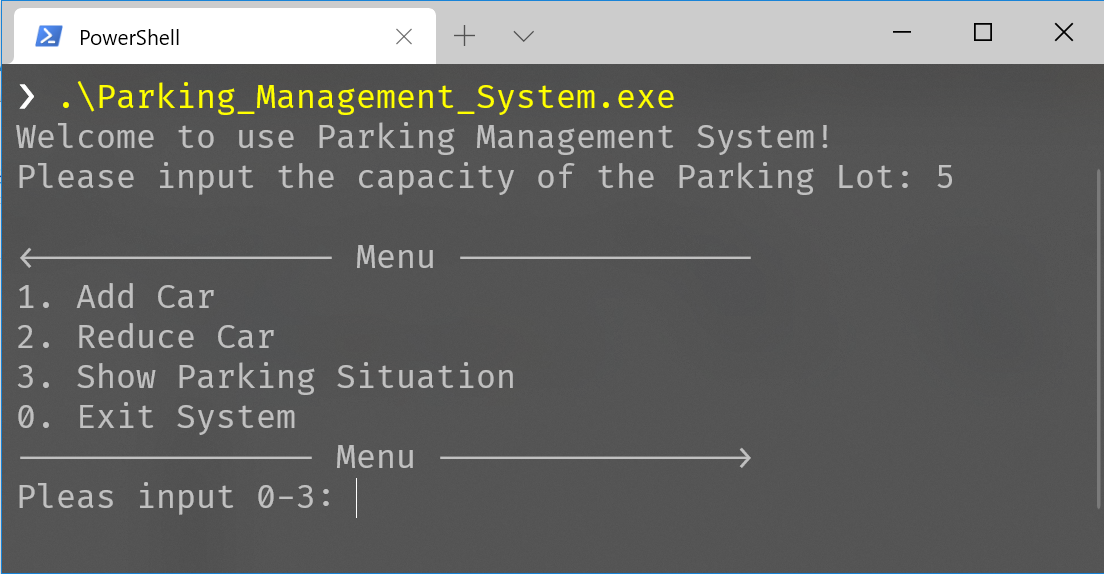
\includegraphics[width=0.7\textwidth]{测试1.png}
        \caption{初始化及菜单}
    \end{figure}


    \begin{figure}
        \centering
        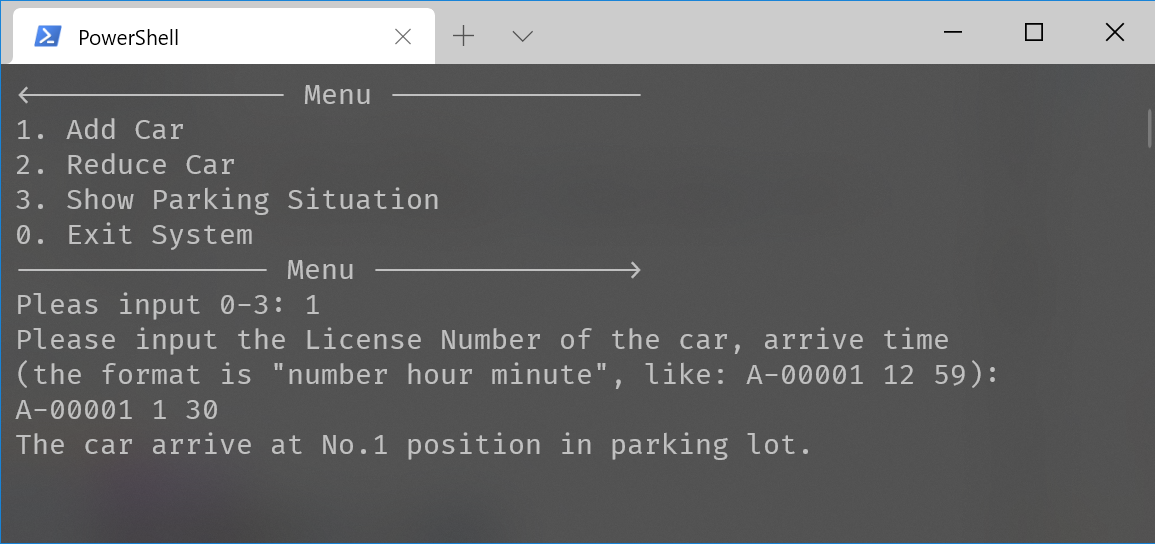
\includegraphics[width=0.75\textwidth]{测试2.png}
        \caption{到达停车场}
        \vspace{1em}
        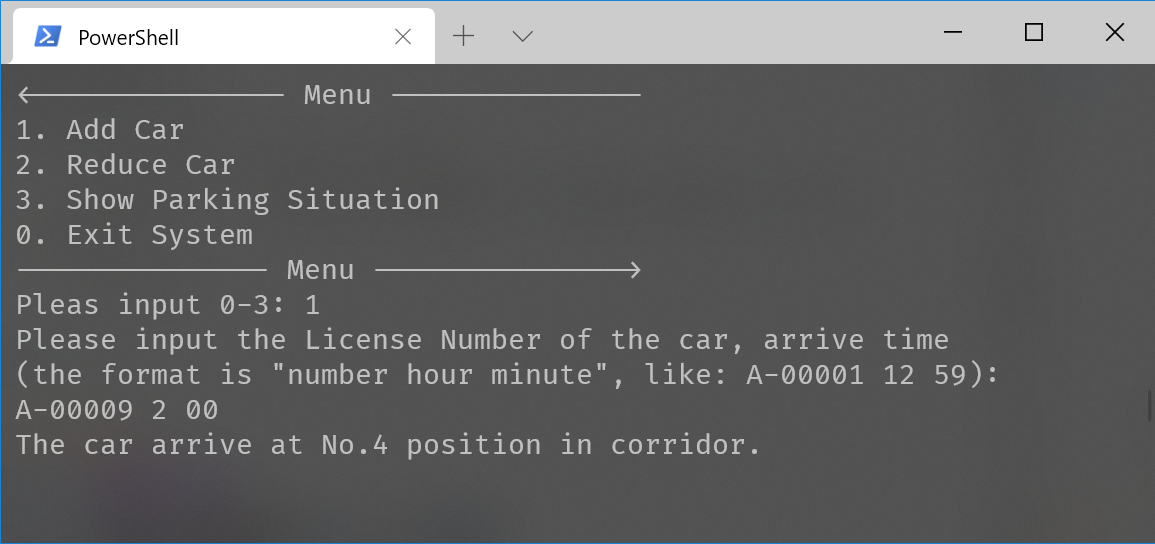
\includegraphics[width=0.75\textwidth]{测试3.png}
        \caption{到达便道}
        \vspace{1em}
        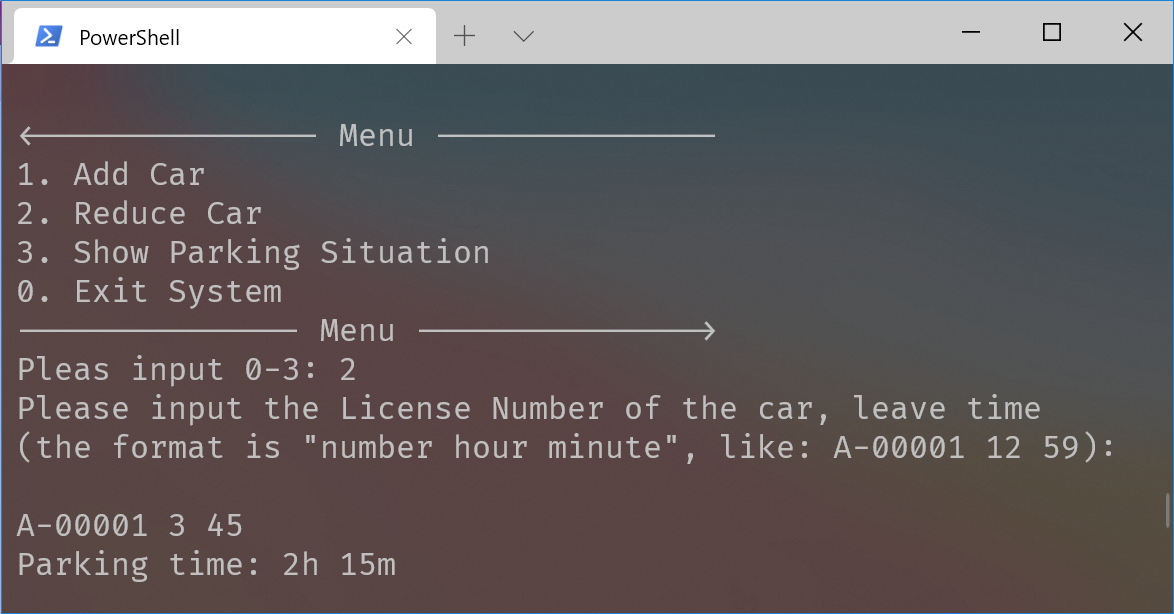
\includegraphics[width=0.75\textwidth]{测试4.png}
        \caption{从停车场离去车辆}
    \end{figure}


    \begin{figure}
        \centering
        \vspace{1em}
        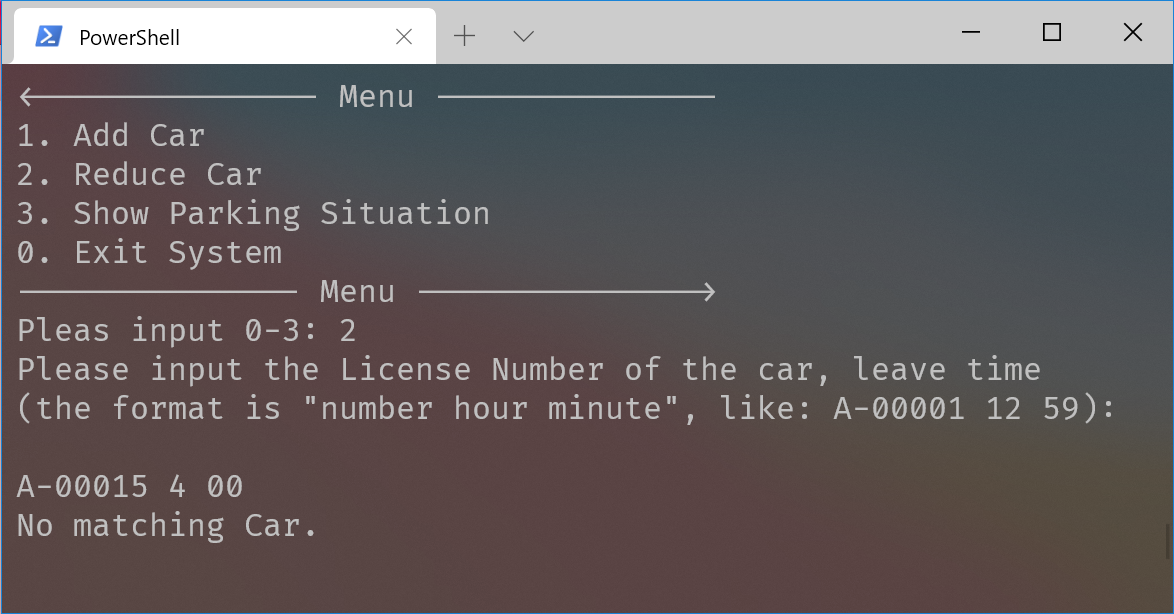
\includegraphics[width=0.75\textwidth]{测试5.png}
        \caption{没有找到车辆}
        \vspace{1em}
        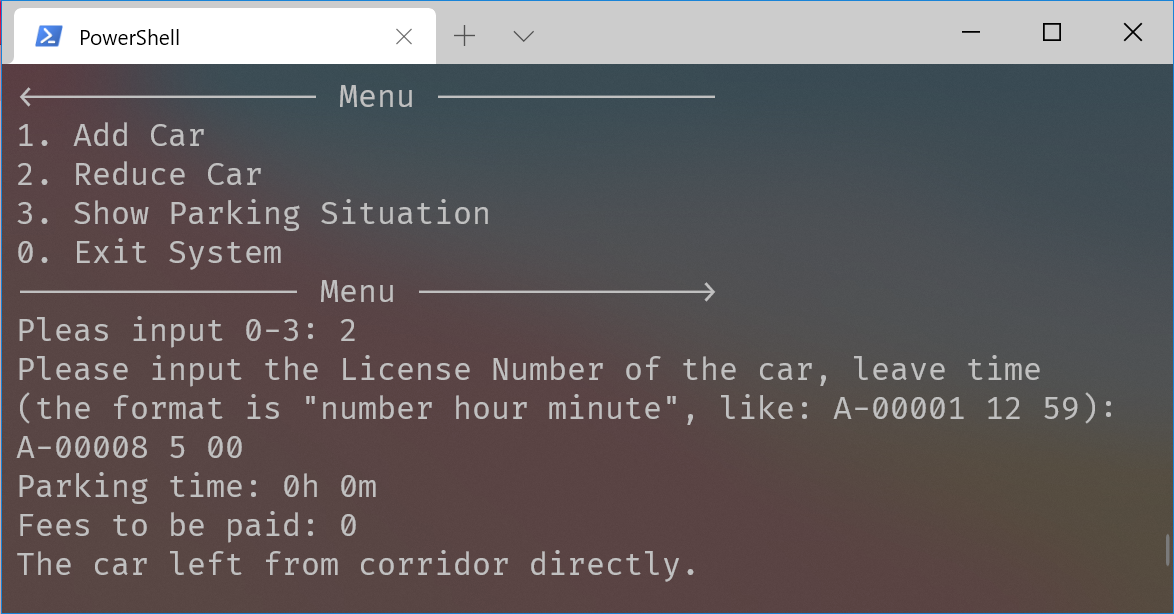
\includegraphics[width=0.75\textwidth]{测试6.png}
        \caption{从便道离去车辆}
        \vspace{1em}
        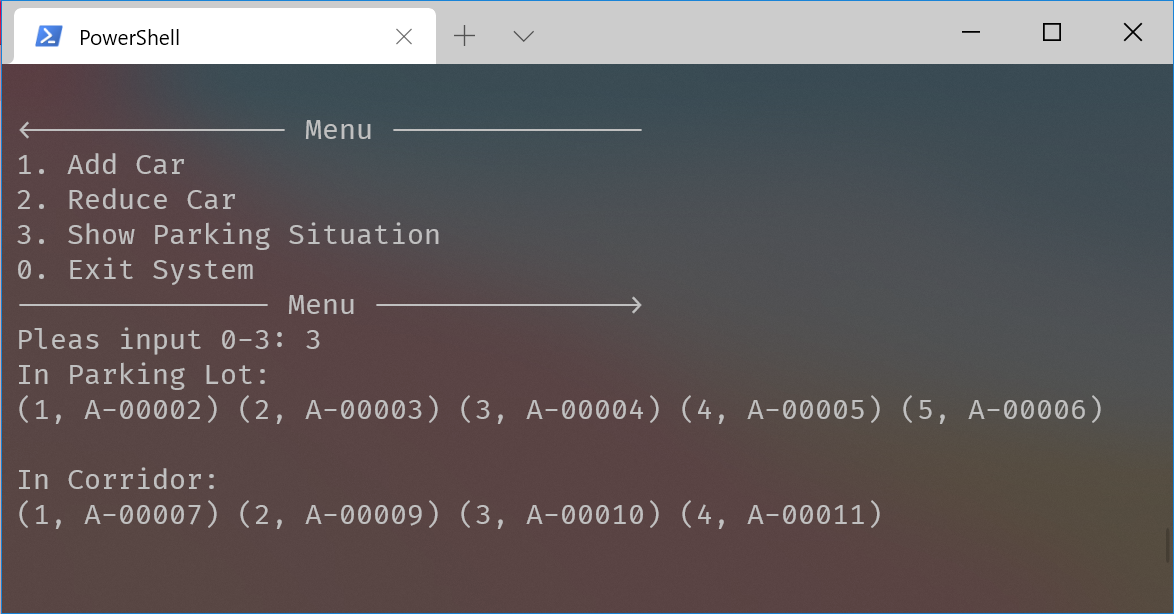
\includegraphics[width=0.75\textwidth]{测试7.png}
        \caption{显示停车情况}
    \end{figure}


    \section{总结}

    通过本次项目实践,熟练地掌握了栈、队列这两种数据结构,并实现了顺序栈、链队列
    模板的编写,增强了编码能力。

    结合栈、队列设计停车场管理系统,使得栈和队列得到实际应用。在实践过程中,需要借助
    栈和队列对停车场内以及便道上的车辆进行有序地调度,增强了离散事件问题的模拟算法设计与求解的能力。
    同时,设计入栈、出栈、入队列、出队列、计时收费等系列算法的设计,对计算机如何模拟实际问题有了
    较好的感性理解。

    此次项目实践,仍有不足之处,如:只设计了一天以内的计时收费,这与生活实际有出入。
    这是项目的改进方向。

    \section{附录}

    本项目实例使用CMake构建,并要求编译器为 G++ ,使用的操作系统是 Windows。

    项目主要文件清单:
    
    \dirtree{%
        .1 /\DTcomment{项目根目录}.
        .2 bin\DTcomment{输出文件夹}.
        .3 Parking\_Management\_System.exe\DTcomment{已经编译的可执行文件}.
        .2 CMakeLists.txt\DTcomment{CMake 项目配置文件}.
        .2 docs\DTcomment{项目文档目录}.
        .3 images\DTcomment{文档使用的图片资源}.
        .3 project2.pdf\DTcomment{项目文档}.
        .3 project2.tex\DTcomment{项目文档\LaTeX 源文件}.
        .2 src\DTcomment{源代码}.
        .3 includes\DTcomment{头文件包含目录}.
        .4 Queue.h\DTcomment{Queue类模板头文件}.
        .4 Stack.h\DTcomment{Stack类模板头文件}.
        .3 Car.h\DTcomment{Time类、Car类头文件}.
        .3 main.cpp\DTcomment{主程序源代码}.
        .3 ParkLot.h\DTcomment{ParkLot类头文件}.
    }

    这些源文件可以在 \url{https://github.com/DianDengJun/Course-Design/tree/main/Winter/Project2} 中查看。
    
    构建本实例的命令(Bash 或 Powershell)如下:
    
    进入根目录,执行:
    
    \begin{verbatim}
        mkdir build
        cd build
        cmake -G "MinGW Makefiles" ..
        make # 或者是 mingw32-make
    \end{verbatim}

    然后进入bin目录运行Parking\_Management\_System.exe。

    \begin{verbatim}
        cd ../bin
        ./Parking_Management_System
    \end{verbatim}

\end{document}